\documentclass[11pt,a4paper]{article}
\usepackage[spanish,es-nodecimaldot]{babel}	% Utilizar español
\usepackage[utf8]{inputenc}					% Caracteres UTF-8
\usepackage{graphicx}						% Imagenes
\usepackage[hidelinks]{hyperref}			% Poner enlaces sin marcarlos en rojo
\usepackage{fancyhdr}						% Modificar encabezados y pies de pagina
\usepackage{float}							% Insertar figuras
\usepackage[textwidth=390pt]{geometry}		% Anchura de la pagina
\usepackage[nottoc]{tocbibind}				% Referencias (no incluir num pagina indice en Indice)
\usepackage{enumitem}						% Permitir enumerate con distintos simbolos
\usepackage[T1]{fontenc}					% Usar textsc en sections
\usepackage{amsmath}						% Símbolos matemáticos
\usepackage{pdflscape}
\usepackage{typearea} % Paginas horizontales

% Comando para poner el nombre de la asignatura
\newcommand{\asignatura}{Sistemas Gráficos}
\newcommand{\autor}{Vladislav Nikolov Vasilev}
\newcommand{\titulo}{Pac-Man 3D}
\newcommand{\subtitulo}{Diseño de la aplicación}
\newcommand{\rama}{Ingeniería del Software}

% Configuracion de encabezados y pies de pagina
\pagestyle{fancy}
\lhead{\autor{}}
\rhead{\asignatura{}}
\lfoot{Grado en Ingeniería Informática}
\cfoot{}
\rfoot{\thepage}
\renewcommand{\headrulewidth}{0.4pt}		% Linea cabeza de pagina
\renewcommand{\footrulewidth}{0.4pt}		% Linea pie de pagina

% new pagestyle
\fancypagestyle{lscape}{
  \headwidth\textwidth
}

\begin{document}
\pagenumbering{gobble}

% Pagina de titulo
\begin{titlepage}

\begin{minipage}{\textwidth}

\centering

%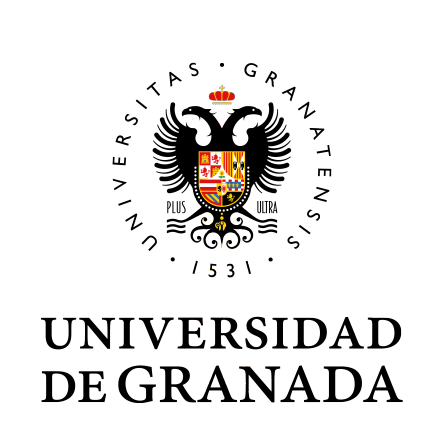
\includegraphics[scale=0.5]{img/ugr.png}\\

\includegraphics[scale=0.3]{img/logo_ugr.jpg}\\[1cm]

\textsc{\Large \asignatura{}\\[0.2cm]}
\textsc{GRADO EN INGENIERÍA INFORMÁTICA}\\[1cm]

\noindent\rule[-1ex]{\textwidth}{1pt}\\[1.5ex]
\textsc{{\Huge \titulo\\[0.5ex]}}
\textsc{{\Large \subtitulo\\}}
\noindent\rule[-1ex]{\textwidth}{2pt}\\[3.5ex]

\end{minipage}

%\vspace{0.5cm}
\vspace{0.7cm}

\begin{minipage}{\textwidth}

\centering

\textbf{Autor}\\ {\autor{}}\\[2.5ex]
\textbf{Rama}\\ {\rama}\\[2.5ex]
\vspace{0.3cm}


\includegraphics[scale=0.3]{img/etsiit.jpeg}

\vspace{0.7cm}
\textsc{Escuela Técnica Superior de Ingenierías Informática y de Telecomunicación}\\
\vspace{1cm}
\textsc{Curso 2019-2020}
\end{minipage}
\end{titlepage}

\pagenumbering{arabic}
\tableofcontents
\thispagestyle{empty}				% No usar estilo en la pagina de indice

% start new page before setting page layout,
% otherwise previous page is also affected
\KOMAoption{paper}{landscape}%
\typearea{12}% sets new DIV

% Establecer pagina horizontal
\recalctypearea
% needed to show page in landscape in viewer
\pdfpageheight=\paperheight
\pdfpagewidth=\paperwidth
% Poner estilo
\pagestyle{lscape}


\setlength{\parskip}{1em}

\section{Diagrama de clases}

\begin{figure}[H]
  \centering
  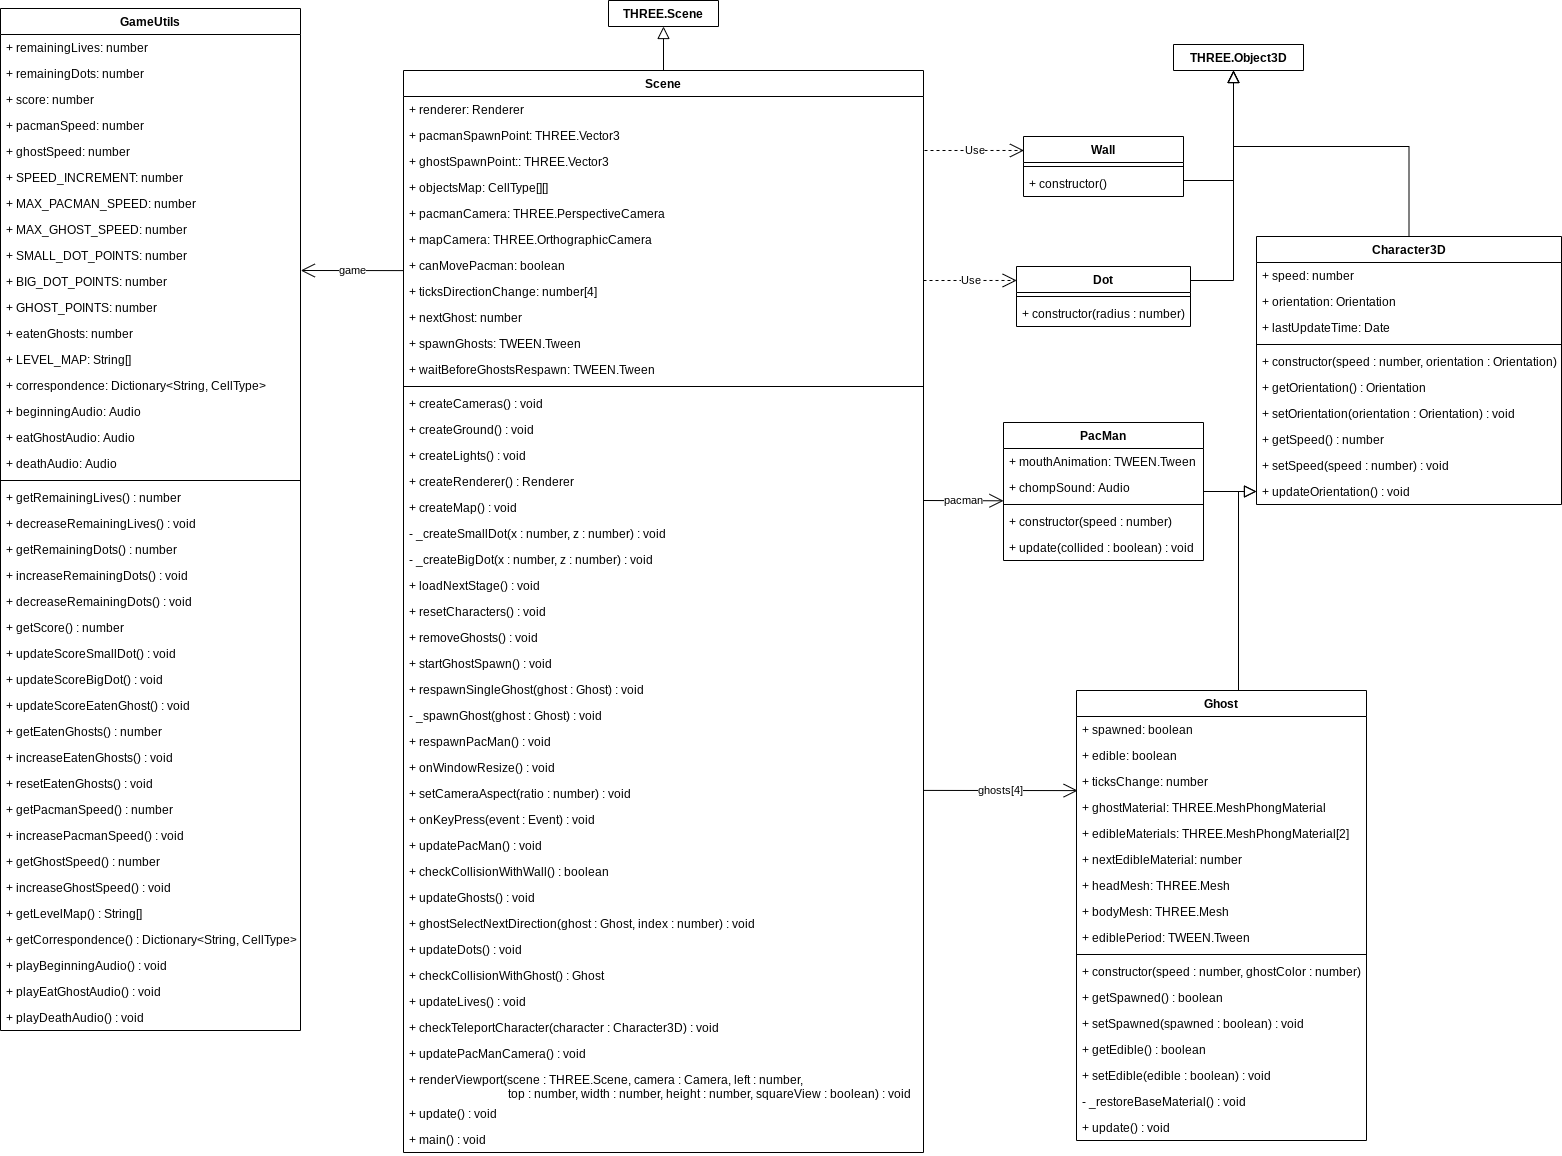
\includegraphics[scale=0.365]{img/diagrama-clases}
\end{figure}

\KOMAoptions{paper=portrait}
\recalctypearea
\pdfpageheight=\paperheight
\pdfpagewidth=\paperwidth
\headwidth\textwidth

Partiendo del diagrama de clases anterior, vamos a describir las clases para que se entienda
qué representa cada una de ellas.

\subsection{Clase \texttt{Character3D}}

Esta clase representa un personaje 3D, heredando de la clase \texttt{THREE.Object3D}. El personaje
tiene un atributo \texttt{speed}, que se refiere a la velocidad a la que se mueve por segundo;
un atributo \texttt{orientation}, que indica hacia donde está orientado el personaje (arriba,
abajo, izquierda o derecha); y un atributo que indica el tiempo en el que se realizó la última
actualización del personaje, es decir, en qué momento se llamó por última vez al método
\texttt{update()} de la clase correspondiente. De esta forma se puede conseguir que los
personajes se muevan de forma independiente a la cantidad de fotogramas que sea capaz de
renderizar el ordenador, tal y como se ha estudiado en clase.

El método más destacable es \texttt{updateOrientation()}. Este método se llama desde el método
\texttt{update()} de las clases derivadas y se encarga de rotar al personaje de manera que mire en
la dirección que le indique el atributo \texttt{orientation}.

\subsection{Clase \texttt{PacMan}}

Esta clase representa al personaje \texttt{Pac-Man}. Hereda de la clase \texttt{Character3D},
con lo cuál hereda sus métodos y atributos. Tiene dos atributos, que son \texttt{mouthAnimation}
y \texttt{chompSound}. El primero es la animación de la boca, la cuál consiste en rotar dos
semiesferas en el eje Z cada una en un sentido. Cuando ambas llegan al final del movimiento,
comienzan a realizarlo en sentido contrario. Dicho movimiento se repite indefinidamente,
deteniéndose solamente cuando el personaje colisiona con un muro. El otro atributo es el sonido
del personaje al moverse. Dicho sonido se reproduce siempre y cuando el personaje se esté
moviendo, es decir, que no haya colisionado con un muro.

El método \texttt{update()} recibe un parámetro, el cuál indica si el personaje ha colisionado
contra un muro (verdadero) o no (falso). En caso de que valga verdadero no se actualiza la
posición del personaje , se detiene la animación de la boca si no estaba ya detenida y se pausa
el sonido del movimiento. En caso contrario, se actualiza la posición en función de la
orientación del personaje, se reproduce el sonido y se actualiza la animación de \texttt{Tween},
continuando con esta o reanudándola en función de si estaba pausada o no anteriormente.

\subsection{Clase \texttt{Ghost}}

Esta clase representa a un fantasma del juego. Hereda de la clase \texttt{Character3D},
con lo cuál hereda sus métodos y atributos. En este caso merece la pena comentar casi todos
los atributos propios, ya que tienen una importancia significativa:

\begin{itemize}
	\item El atributo \texttt{spawned} es un booleano que indica si el fantasma ha aparecido en
	el escenario o no.
	\item El atributo \texttt{edible} indica si el fantasma es comestible o no.
	\item \texttt{ticksChange} es un atributo que se utiliza en la animación que se
	lanza cuando el fantasma es comestible. Básicamente, una vez que haya pasado el 70\%
	del tiempo de la animación, cada 100 \textit{ticks} o actualizaciones de la animación
	el material del fantasma va a ir cambiando, dando la sensación de intermitencia. El material
	va a ir cambiando entre el azul oscuro y el blanco.
	\item \texttt{ghostMaterial} es el material base del fantasma.
	\item El atributo \texttt{edibleMaterials} es un \textit{array} que contiene los 
	dos materiales que tiene el fantasma mientras puede ser comido: el azul oscuro y el blanco.
	\item El atributo \texttt{nextEdibleMaterial} es el índice del siguiente material que se
	va a utilizar en la animación. Empieza con el valor 0, refiriéndose por tanto al azul
	oscuro, y después se incrementa para hacer referencia al blanco. Después va cambiando de
	valor cada 100 \textit{ticks} como se ha explicado anteriormente.
	\item \texttt{bodyMesh} y \texttt{headMesh} son los \textit{mesh} que forman el cuerpo
	y la cabeza del fantasma, respectivamente. Es necesario guardarlos, ya que el material
	de estos se va a ver modificado cuando el fantasma pasa a ser comestible y cuando deja
	de serlo.
	\item Por último, \texttt{edibleMaterial} es la animación que controla el momento en el
	que el fantasma es comestible. Tiene una duración de 8 segundos y se activa cuando el
	\texttt{Pac-Man} se come un punto grande. Puede terminar antes de los 8 segundos si el
	jugador se come al fantasma. Una vez que se acaba, el fantasma deja de ser comestible.
\end{itemize}

La clase tiene un par de \textit{setters} y \textit{getters}, además del método
\texttt{update()}, el cuál se encarga de controlar el movimiento del fantasma en función de
la orientación. No obstante, de todos ellos destacan dos. Uno de ellos es
\texttt{setEdible(edible)} el cuál cambia el valor del atributo \texttt{edible} e inicia o
detiene la animación \texttt{ediblePeriod} en función de dicho valor, además de establecer el
material del fantasma al correspondiente y de inicializar otros valores, como por ejemplo
\texttt{nextEdibleMaterials} y \texttt{ticksChange}. El otro es \texttt{\_restoreBaseMaterial()},
el cuál, como su propio nombre indica, restaura el material base del fantasma. Este es un
método auxiliar utilizado por el anterior y por la animación una vez que esta haya sido
completada.

\subsection{Clase \texttt{Wall}}

Esta clase hereda de \texttt{THREE.Object3D} y representa un muro del juego, el cuál es de color
azul oscuro. Su constructor simplemente crea una caja de tamaño $1 \times 1 \times 1$ y la
posiciona sobre el suelo.

\subsection{Clase \texttt{Dot}}

Esta clase hereda de \texttt{THREE.Object3D} y representa o bien un punto pequeño o uno grande
en función del radio que se utilice a la hora de crear un \textit{mesh}. Un punto pequeño tiene
un radio de $0.1$ unidades, mientras que uno grande tiene un radio de $0.2$ unidades.

\subsection{Clase \texttt{GameUtils}}

Esta es una clase que contiene toda la información del juego: puntuación del jugador, puntuación
que proporciona cada elemento del juego, número de fantasmas que se ha comido el jugador
mientras estos son comestibles, vidas restantes, puntos restantes en el mapa por comer,
velocidades de los personajes y sus velocidades máximas, audios que se utilizan en determinados
momentos de la partida (inicio de la partida, al comerse a un fantasma y al morir) y el mapa del
juego junto con su correspondencia a tipos de celdas.

La mayoría de sus métodos son \textit{getters}, además de tener otros métodos que le
permiten modificar algunos de los atributos. Hay unos pocos que son de especial interés, como
podría ser el caso de los métodos que incrementan la velocidad de los personajes, ya que
comprueban que no se ha superado el máximo antes. El incremento de velocidad es de $0.5$ cada
vez que se completa un nivel. La velocidad inicial del \texttt{Pac-Man} es de 3 unidades por
segundo, mientras que la de los fantasmas es de $2.5$. La velocidad máxima del \texttt{Pac-Man} es
de $5.5$ unidades por segundo, mientras que la de los fantasmas es de 5. De esta forma, el
personaje siempre es algo más rápido que los fantasmas.

Otro método interesante es el de aumentar la puntuación del jugador cuando se ha comido a un
fantasma. Recordemos que el primer fantasma proporciona 200 puntos, el segundo 400, el tercero 800
y el cuarto 1600. Para obtener estos valores se utiliza la siguiente fórmula:

\begin{equation}
score_{ghost} = 2^{eatenGhosts - 1} \times GHOST\_POINTS
\end{equation}

\noindent donde \texttt{GHOST\_POINTS} es la puntuación base de un fantasma, la cuál es de 200.
El restulado de esa expresión se suma a la puntuación del jugador.

\subsection{Clase \texttt{Scene}}

Esta es la clase que contiene la escena 

\newpage

\begin{thebibliography}{5}

\bibitem{nombre-referencia}
Texto referencia
\\\url{https://url.referencia.com}

\end{thebibliography}

\end{document}

